\documentclass{article}
\usepackage{graphicx} % Required for inserting images
\usepackage{url}
\usepackage{amssymb}
\usepackage[T1]{fontenc} 
\usepackage{minted}
\usepackage{float}
\usepackage{amsmath}
\usepackage{subcaption}

\title{Audio Analyzer - Piano Tuner}
\author{Yaniv Arbel, Bar Maman, Gilad Bregman}
\date{December 2024}

\begin{document}

\maketitle

\section*{Abstract}

In this paper, we will Analyze sound audio recordings. Since sound is inherently a wave phenomena, we will choose Fourier Transform to convert the recording to its frequency components. We will show how efficient the Fourier approximation is to extract frequencies out of an audio recording and create a algorithm that helps the user to tune their instrument. 

\section*{Table of Content}
\begin{enumerate}
    \item Introduction
    \item Fourier Mathematics
    \begin{itemize}
        \item Fourier Series
        \item Euler's Formula and Complex Numbers
        \item Transition to Discrete Fourier Transform (DFT/FFT)
    \end{itemize}
    \item Notes Analysis
    \begin{itemize}
        \item Dominant Notes Extraction Using FFT
        \item Example of Use - Jingle Bells (Christmas song)
        \item Tuning a Note
    \end{itemize}
    \item Conclusion
    \item References
    \item Code References
\end{enumerate}


\section*{Introduction}
"The Fourier transform has become the cornerstone of computational mathematics"$^{[1]}$ that allows the decomposition of complex functions into their fundamental frequency components. "Fourier introduced the concept that sine and cosine functions of increasing frequency provide an orthogonal basis for the space of solution functions"$^{[1]}$. This transformative approach is not merely a theoretical construct but a practical tool with applications spanning different fields of processing data. By converting a time-domain signal, such as sound waves, into its frequency-domain representation, the Fourier Transform reveals the underlying structure of the signal and allows us to create a large system of equations that describe an audio recording.

The ability to approximate any function using the Fourier series positions it as a universal tool in analysis. In the context of sound waves, the Fourier Transform's utility becomes even more evident. In fact, "The DFT is one of the main mathematical workhorses of signal processing," and the FFT (the computational method of the DFT) is "considered to be one of the most influential and important algorithmic developments of the 20th century."$^{[6]}$ The use of the Fourier Transform methods "has greatly increased the effectiveness of digital methods for a very wide range of problems such as spectral analysis, signal processing, Fourier spectroscopy, image processing, and the solution of differential equations."$^{[4]}$ For example, "Shazam achieves a representation that is robust to noise distortions," and is initially using "the fundamental concept of the Fourier Transform."$^{[5]}$


An important feature of the algorithm is its linearity. "Another way to view the Fourier Transform is as an operator acting on the space of functions: Let $f : \mathbb{R} \to \mathbb{R}$ be a function for which  
$\int_{-\infty}^\infty |f(t)| \, dt < \infty$. 

That is, for each $f$, the operator  $\mathcal{F}$  maps $f$ to the function $\mathcal{F}f$."$^{[5]}$

Therefore, its behavior can be described and analyzed using the tools and principles of linear algebra when dealing with large systems of equations.

However, "with the emergence of big data problems, in which the size of the processed data sets can easily exceed terabytes, the FFT is not always fast enough.$^{[6]}$" For example, in medical imaging, it is highly desirable to reduce the time that the patient spends in a magnetic resonance imaging machine. This motivates the need for algorithms that can compute the Fourier transform in sublinear time (in an amount of time that is considerably smaller than the size of the data),and that use only a subset of the input data."$^{[6]}$

Therefore, our goal is to demonstrate that, by applying the Fourier Transform to extract the frequency components of a recording, in our case piano notes, we can utilize only the dominant components to reduce the data and even tune a note to its target frequency.

\section*{Fourier Mathematics}
For our Purposes, Fourier Transform is a coordinate transformation that is useful  for representing data.$^{[1]}$ It is derived particularly for approximating partial differential equations, which is relevant for representing sounds waves.$^{[1]}$ It is generally "the most straightforward" and "utilized way of extracting frequencies from a stationary signal, and the intrinsic advantage of this approach is that one can separately extract the frequencies for any desired spectral range"$^{[8]}$.
\begin{itemize}
    \item{ 
    \section*{Fourier Series}

    The following data was studied from the textbook \textit{Data-Driven Science and Engineering}, by Brunton, Steven L., and J. Nathan Kutz$^{[1]}$.\\\\ 
    Using a Fourier series expansion, we will approximate a function \( f(x) \).  
    The Fourier series representation decomposes \( f(x) \) into a series of cosine and sine functions at different frequencies \( k \).  
    The Fourier series for a function \( f(x) \) is given by:

    \[
    f(x) \approx \frac{A_0}{2} + \sum_{k=1}^{\infty} \left(A_k \cos(kx) + B_k \sin(kx)\right)
    \]

    Here, the Fourier Series expresses \( f(x) \) as a linear combination of the basis functions \( \cos(kx) \) and \( \sin(kx) \).  

    The coefficients \( A_k \) and \( B_k \) represent the amplitudes of the cosine and sine terms at each frequency \( k \).  
    These coefficients are determined by projecting \( f(x) \) onto the cosine and sine basis functions.
    
    As an example we will first define a function f(x):
    \begin{minted}[frame=lines, fontsize=\small]{python}
    # Define a hat function
    def hat_function(x):
        return np.where(np.abs(x) <= 1, 1 - np.abs(x), 0)  
    # Define x values
    x_values = np.linspace(-3, 3, 1000)
    \end{minted}
    
    \begin{figure}[H] 
    \centering
    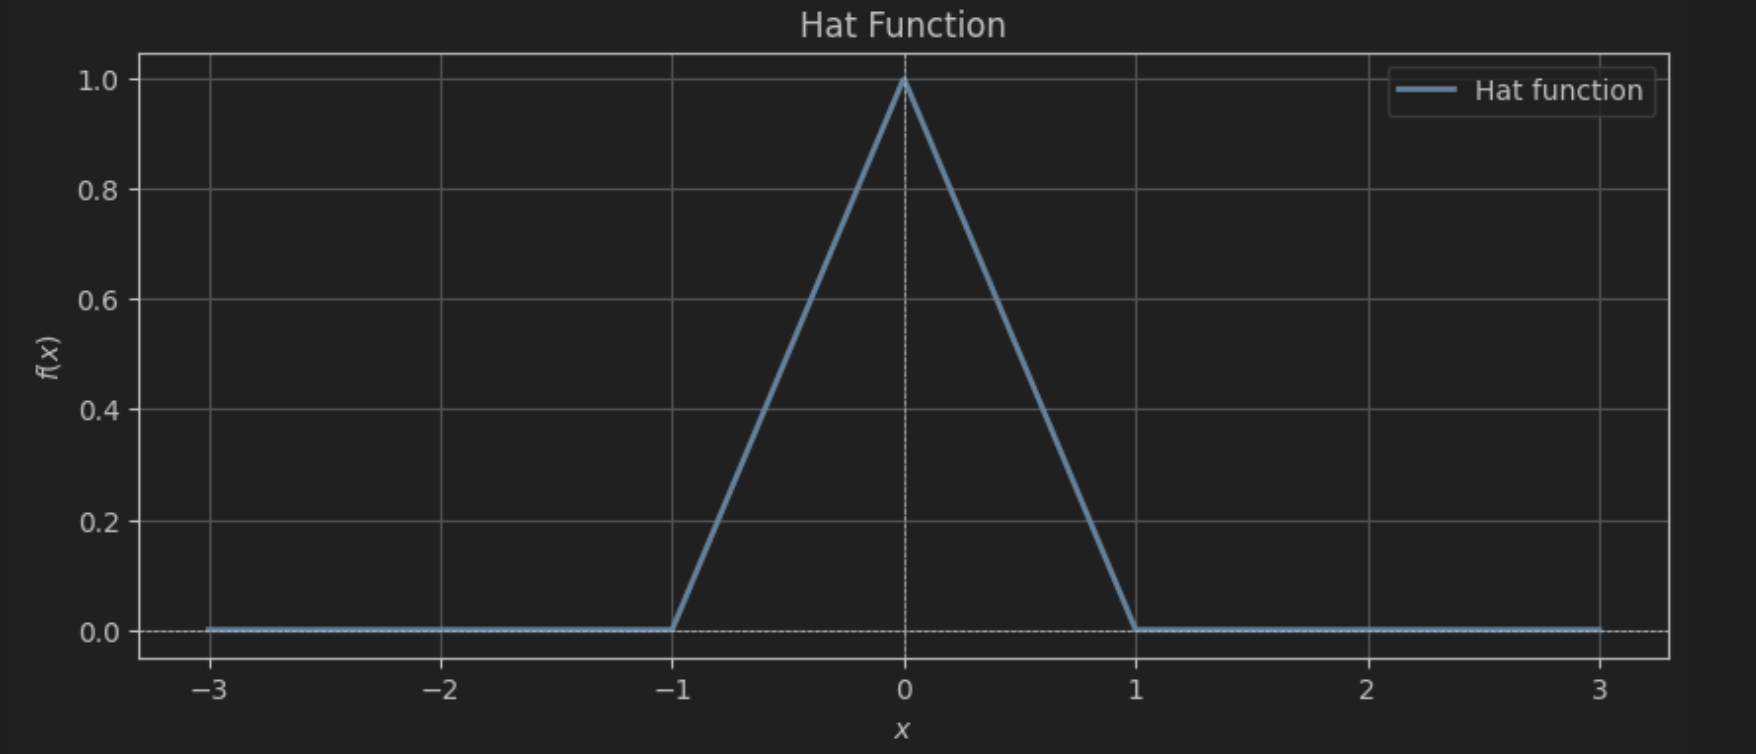
\includegraphics[width=0.8\textwidth]{image1.png}
    \caption{Graph of the Hat Function \( f(x) \).}
    \label{fig:hat_function}
    \end{figure}
    
    Using Fourier Series we approximate 5 coefficients form the defined $f(x)$ hat function as follows.

    
    \begin{minted}[frame=lines, fontsize=\small]{python}
    # here we define the periodic extension of the hat function in periods of 2 pi
def f(x):
    x = np.mod(x + np.pi, 2 * np.pi) - np.pi
    return np.where(np.abs(x) <= 1, 1 - np.abs(x), 0)
N = 5  # Number of terms in the Fourier series
x_values = np.linspace(-2 * np.pi, 2 * np.pi, 1000) 

# Calculate the Fourier coefficients
def compute_coefficients(N):
    A0 = (1 / (2 * np.pi)) * trapezoid(f(x_values), x_values)  # A0 coefficient
    A_k = []
    B_k = []

    for k in range(1, N + 1):
        # Compute Ak
        cos_terms = f(x_values) * np.cos(k * x_values)
        Ak = (1 / np.pi) * trapezoid(cos_terms, x_values)
        A_k.append(Ak)

        # Compute Bk
        sin_terms = f(x_values) * np.sin(k * x_values)
        Bk = (1 / np.pi) * np.trapezoid(sin_terms, x_values)
        B_k.append(Bk)

    return A0, np.array(A_k), np.array(B_k)

# Reconstruct the Fourier series
def fourier_series(x, A0, A_k, B_k):
    result = A0 / 2 
    terms = [A0 / 2] 
    for k in range(1, len(A_k) + 1):
        term = A_k[k - 1] * np.cos(k * x) + B_k[k - 1] * np.sin(k * x)
        result += term
        terms.append(term)
    return result, terms

# Compute coefficients and reconstruct the Fourier series
A0, A_k, B_k = compute_coefficients(N)
f_approx, terms = fourier_series(x_values, A0, A_k, B_k)
    
    \end{minted}
     \begin{figure}[H] 
    \centering
    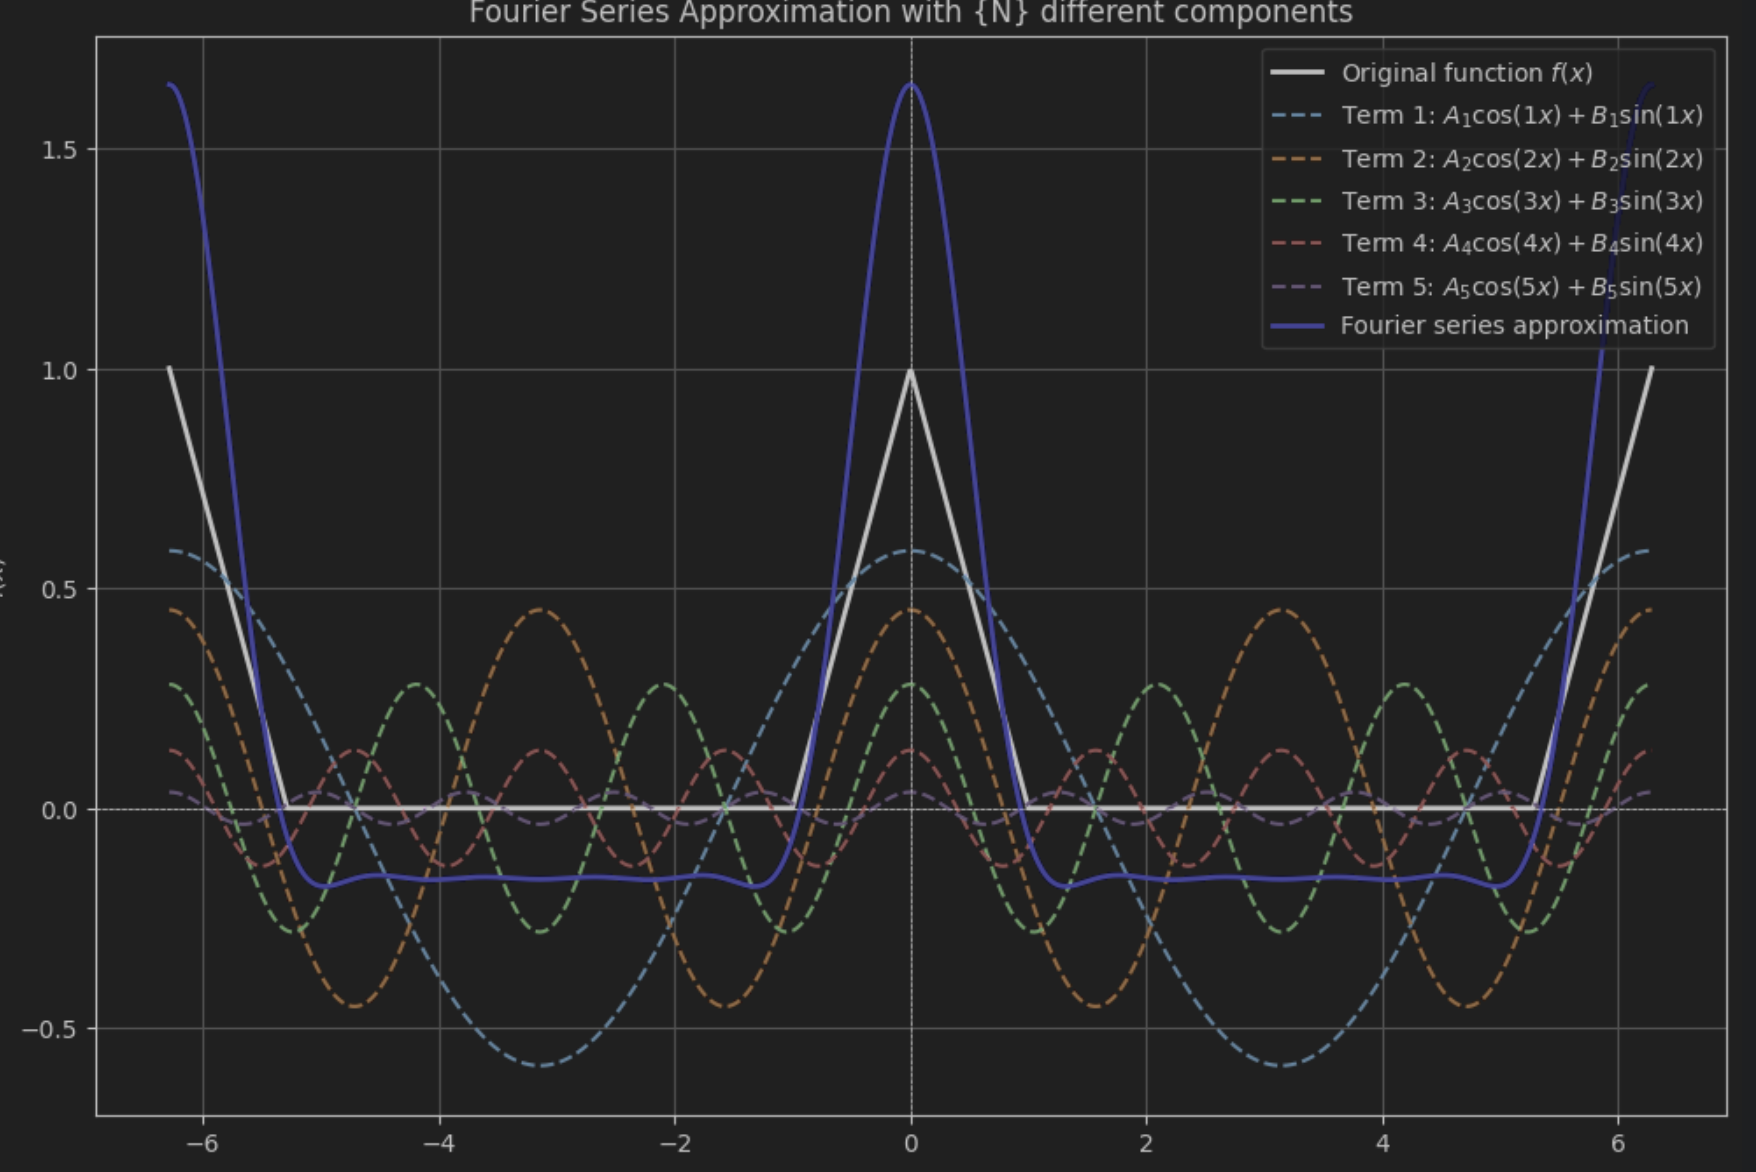
\includegraphics[width=0.8\textwidth]{image2.png}
    \caption{Graph of the Hat Function approximation with 5 terms.}
    \label{fig:hat_function}
    \end{figure}
    
    The coefficients \( A_k \) and \( B_k \) are calculated by taking the inner product of \( f(x) \) with the cosine and sine basis functions.  
    This projection extracts the contribution of each frequency component. \\

    As learned in class, this process is similar to projecting the vector $X$ onto orthogonal basis vector $u_i$

    The vector $X$ corresponds to the function $f(x)$ and the basis vector $u_i$ is corresponds to the sine and cosine functions $cos(kx)$ and $sine(kx)$ which form an orthogonal basis: 

    Therefore, 
\[
\mathbf{X} = t_1 \mathbf{u}_1 + t_2 \mathbf{u}_2 + \dots + t_n \mathbf{u}_n
\]

Then, when taking the inner product of \( \mathbf{u}_i \) with \( \mathbf{X} \):
\[
\mathbf{u}_i \cdot \mathbf{X} = \mathbf{u}_i \cdot (t_1 \mathbf{u}_1 + t_2 \mathbf{u}_2 + \dots + t_n \mathbf{u}_n)
\]
Apply the the dot product:
\[
\mathbf{u}_i \cdot \mathbf{X} = t_1 (\mathbf{u}_i \cdot \mathbf{u}_1) + t_2 (\mathbf{u}_i \cdot \mathbf{u}_2) + \dots + t_n (\mathbf{u}_i \cdot \mathbf{u}_n)
\]
$\mathbf{u}_i \cdot \mathbf{u}_j = 0 \quad \text{for} \quad i \neq j$, and
This reduces the expression to:
\[
\mathbf{u}_i \cdot \mathbf{X} = t_i (\mathbf{u}_i \cdot \mathbf{u}_i) = t_i \|\mathbf{u}_i\|^2
\]
Since we want to solve for \( t_i \):
\[
t_i = \frac{\mathbf{u}_i \cdot \mathbf{X}}{\|\mathbf{u}_i\|^2}
\]
This is analogous to finding:
\[
\langle \cos(kx), f(x) \rangle = \left\langle \sum_{k=0}^\infty \left(A_k \cos(kx) + B_k \sin(kx)\right), \cos(kx) \right\rangle
\]

\[
\langle \sin(kx), f(x) \rangle = \left\langle \sum_{k=0}^\infty \left(A_k \cos(kx) + B_k \sin(kx)\right), \sin(kx) \right\rangle
\]

Then applying this on the Fourier Series, where the inner product of two functions \( f \) and \( g \) over an interval \([a, b]\) is defined as:
    \[
    \langle f, g \rangle = \int_{a}^{b} f(x) g(x) \, dx
    \]

    To obtain \( A_k \) and \( B_k \), we take the inner products:

    \[
    A_k = \frac{\langle f, \cos(kx) \rangle}{||\cos(kx)||^2}, \quad B_k = \frac{\langle f, \sin(kx) \rangle}{||\sin(kx)||^2}
    \]

    where \( ||g||^2 = \langle g, g \rangle \) is the norm squared of the basis function.  
    This normalization ensures each coefficient accurately represents the component of \( f(x) \) in that basis direction.\\

    Fourier Coefficients on \([- \pi, \pi]\):
    To compute the Fourier coefficients, we normalize the inner product by dividing by the interval length \( 2\pi \).  
    For \( A_k \) and \( B_k \), we use:

    \[
    A_k = \frac{1}{\pi} \int_{-\pi}^{\pi} f(x) \cos(kx) \, dx, \quad 
    B_k = \frac{1}{\pi} \int_{-\pi}^{\pi} f(x) \sin(kx) \, dx
    \]

    The normalization factor \( \frac{1}{\pi} \) accounts for the interval length \( 2\pi \), as the integral itself spans this length.  
    The norm squared of the basis functions \( \cos(kx) \) and \( \sin(kx) \) over \([- \pi, \pi]\) is given by:

    \[
    ||\cos(kx)||^2 = \langle \cos(kx), \cos(kx) \rangle = \int_{-\pi}^\pi \cos^2(kx) \, dx = \pi,\] \\
    \[
    ||\sin(kx)||^2 = \langle \sin(kx), \sin(kx) \rangle = \int_{-\pi}^\pi \sin^2(kx) \, dx = \pi
    \]

    When dividing \( \langle f, \cos(kx) \rangle \) by \( ||\cos(kx)||^2 \), the coefficient \( A_k \) becomes:

    \[
    A_k = \frac{1}{\pi} \int_{-\pi}^\pi f(x) \cos(kx) \, dx
    \]

    Similarly, \( B_k \) is normalized as:

    \[
    B_k = \frac{1}{\pi} \int_{-\pi}^\pi f(x) \sin(kx) \, dx
    \]\\
    
    Fourier Series for the Interval [0, L]

The Fourier series for a function \( f(x) \) defined on the interval \([0, L]\) is given by:

\[
f(x) \approx \frac{A_0}{2} + \sum_{k=1}^\infty \left( A_k \cos\left(\frac{2\pi k x}{L}\right) + B_k \sin\left(\frac{2\pi k x}{L}\right) \right)
\]

Fourier Coefficients on \([0, L]\):

The Fourier coefficients for the interval \([0, L]\) are calculated as follows:

\[
A_0 = \frac{2}{L} \int_0^L f(x) \, dx
\]
\[
A_k = \frac{2}{L} \int_0^L f(x) \cos\left(\frac{2\pi k x}{L}\right) \, dx
\]
\[
B_k = \frac{2}{L} \int_0^L f(x) \sin\left(\frac{2\pi k x}{L}\right) \, dx
\]

The factor \( \frac{2}{L} \) normalizes the interval length \( L \), replacing \( \frac{1}{\pi} \) for the interval \([- \pi, \pi]\). The arguments of the cosine and sine functions, scaled by \( \frac{2\pi}{L} \), reflect the interval's length.\\

Matrix Representation of Basis Functions:

The cosine and sine basis functions can be represented as separate matrices:

\[
G_{\cos} = \begin{bmatrix}
\cos(x_1) & \cos(2x_1) & \dots & \cos(Nx_1) \\
\cos(x_2) & \cos(2x_2) & \dots & \cos(Nx_2) \\
\vdots & \vdots & & \vdots \\
\cos(x_M) & \cos(2x_M) & \dots & \cos(Nx_M)
\end{bmatrix}
\]
\[
G_{\sin} = \begin{bmatrix}
\sin(x_1) & \sin(2x_1) & \dots & \sin(Nx_1) \\
\sin(x_2) & \sin(2x_2) & \dots & \sin(Nx_2) \\
\vdots & \vdots & & \vdots \\
\sin(x_M) & \sin(2x_M) & \dots & \sin(Nx_M)
\end{bmatrix}
\]

Here, \( M \) is the number of sample points, and \( N \) is the number of frequencies used. The size of each matrix is \( M \times N \).\\

Fourier Coefficients in Matrix Form:

The Fourier coefficients are computed using the inner product in matrix form:

\[
\mathbf{A} = \frac{1}{\pi} G_{\cos}^\top \mathbf{f}, \quad \mathbf{B} = \frac{1}{\pi} G_{\sin}^\top \mathbf{f}
\]

where \( \mathbf{A} = [A_1, A_2, \dots, A_N]^\top \) and \( \mathbf{B} = [B_1, B_2, \dots, B_N]^\top \) are the cosine and sine coefficients, respectively. The vector \( \mathbf{f} = [f(x_1), f(x_2), \dots, f(x_M)]^\top \) represents the sampled function values.\\

Matrix Representation of the Inner Product:

The inner product calculation can also be expressed as:

\[
c_{jk} = \sum_i G_{ij} f_i
\]\\

Fourier Series Approximation for the Interval [0, L]

The Fourier series approximation of \( f(x) \) on \([0, L]\) is given by:

\[
f(x) \approx \frac{A_0}{2} + \sum_{k=1}^N \left( A_k \cos\left(\frac{2\pi k x}{L}\right) + B_k \sin\left(\frac{2\pi k x}{L}\right) \right)
\]

The cosine and sine matrices for the interval \([0, L]\) become:

\[
G_{\cos} = \begin{bmatrix}
\cos\left(\frac{2\pi x_1}{L}\right) & \cos\left(\frac{4\pi x_1}{L}\right) & \dots & \cos\left(\frac{2\pi N x_1}{L}\right) \\
\cos\left(\frac{2\pi x_2}{L}\right) & \cos\left(\frac{4\pi x_2}{L}\right) & \dots & \cos\left(\frac{2\pi N x_2}{L}\right) \\
\vdots & \vdots & & \vdots \\
\cos\left(\frac{2\pi x_M}{L}\right) & \cos\left(\frac{4\pi x_M}{L}\right) & \dots & \cos\left(\frac{2\pi N x_M}{L}\right)
\end{bmatrix}
\]
\[
G_{\sin} = \begin{bmatrix}
\sin\left(\frac{2\pi x_1}{L}\right) & \sin\left(\frac{4\pi x_1}{L}\right) & \dots & \sin\left(\frac{2\pi N x_1}{L}\right) \\
\sin\left(\frac{2\pi x_2}{L}\right) & \sin\left(\frac{4\pi x_2}{L}\right) & \dots & \sin\left(\frac{2\pi N x_2}{L}\right) \\
\vdots & \vdots & & \vdots \\
\sin\left(\frac{2\pi x_M}{L}\right) & \sin\left(\frac{4\pi x_M}{L}\right) & \dots & \sin\left(\frac{2\pi N x_M}{L}\right)
\end{bmatrix}
\]
}

\item{ \section*{Euler's Formula and Complex Numbers$^{[1]}$}

\textbf{Representation of Complex Numbers:}

A complex number \( z \) can be represented in Cartesian form as:
\[ z = x + iy, \quad \text{where \( x \) is the real part and \( y \) is the imaginary part.} \]
In polar coordinates, we relate \( x \) and \( y \) to the magnitude \( R \) and angle \( \theta \):
\[ x = R \cos(\theta), \quad y = R \sin(\theta). \]
Using these relations, the complex number can be expressed as:
\[ z = R (\cos(\theta) + i \sin(\theta)). \]
Using Euler's formula, we rewrite this as:
\[ z = R e^{i\theta}, \quad \text{where \( R = \sqrt{x^2 + y^2} \) is the magnitude, and \( \theta = \arctan\left(\frac{y}{x}\right) \) is the angle.} \]

\textbf{Properties of Complex Numbers in Polar Form:}

For two complex numbers \( z_1 = R_1 e^{i\theta_1} \) and \( z_2 = R_2 e^{i\theta_2} \):
\begin{align*}
\text{Multiplication: } & z_1 z_2 = R_1 R_2 e^{i(\theta_1 + \theta_2)}, \\
\text{Division: } & \frac{z_1}{z_2} = \frac{R_1}{R_2} e^{i(\theta_1 - \theta_2)}.
\end{align*}

\textbf{Taylor Series Expansions of Exponentials, Sine, and Cosine:}

The Taylor expansion for \( e^x \) is:
\[ e^x = \sum_{k=0}^\infty \frac{x^k}{k!}, \quad \text{where \( x \in \mathbb{C} \)}. \]
For the complex exponential \( e^{ix} \), the series becomes:
\[ e^{ix} = \sum_{k=0}^\infty \frac{(ix)^k}{k!} = 1 + ix - \frac{x^2}{2!} - i\frac{x^3}{3!} + \frac{x^4}{4!} + \dots \]
Grouping terms into real and imaginary parts:
\[ e^{ix} = \left( 1 - \frac{x^2}{2!} + \frac{x^4}{4!} - \dots \right) + i \left( x - \frac{x^3}{3!} + \frac{x^5}{5!} - \dots \right). \]
These real and imaginary parts correspond to the Taylor series for \( \cos(x) \) and \( \sin(x) \), respectively:
\begin{align*}
\cos(x) &= \sum_{n=0}^\infty \frac{(-1)^n x^{2n}}{(2n)!}, \\
\sin(x) &= \sum_{n=0}^\infty \frac{(-1)^n x^{2n+1}}{(2n+1)!}.
\end{align*}
Thus, we derive Euler's formula:
\[ e^{ix} = \cos(x) + i \sin(x). \]

\textbf{The Benefits of Euler's Formula:}

Using Euler's formula, we can represent trigonometric functions in terms of exponentials:
\begin{align*}
\cos(x) &= \frac{e^{ix} + e^{-ix}}{2}, \\
\sin(x) &= \frac{e^{ix} - e^{-ix}}{2i}.
\end{align*}
This reduces the need to compute separate sine and cosine terms, simplifying calculations.

\textbf{The Role of the Conjugate in Fourier Analysis:}

The complex conjugate of a complex number \( z = a + bi \) is \( \overline{z} = a - bi \). For exponentials, the conjugate is:
\[ \overline{e^{ix}} = e^{-ix}, \quad \text{which corresponds to flipping the sign of the imaginary part.} \]
The complex conjugate is essential in Fourier analysis when computing the Fourier coefficients:
\[ C_k = \frac{1}{L} \int_0^L f(x) \overline{e^{i \frac{2\pi k x}{L}}} \, dx. \]
Since \( \overline{e^{i \theta}} = e^{-i \theta} \), this ensures that the inner product isolates the contribution of the \( k \)-th mode:
\[
\int_0^L e^{i \frac{2\pi j x}{L}} \overline{e^{i \frac{2\pi k x}{L}}} \, dx = 
\begin{cases} 
L, & \text{if } j = k, \\
0, & \text{if } j \neq k.
\end{cases}
\]
This orthogonality property simplifies the computation of Fourier coefficients \( C_k \), reducing redundant calculations.

\textbf{Fourier Series for \([0, L]\):}

For a general interval \([0, L]\), the Fourier series for a function \( f(x) \) is defined as:
\[ f(x) \approx \frac{A_0}{2} + \sum_{k=1}^\infty \left( A_k \cos\left(\frac{2\pi k x}{L}\right) + B_k \sin\left(\frac{2\pi k x}{L}\right) \right). \]

The Fourier coefficients are given by:
\begin{align*}
A_0 &= \frac{2}{L} \int_0^L f(x) \, dx, \\
A_k &= \frac{2}{L} \int_0^L f(x) \cos\left(\frac{2\pi k x}{L}\right) \, dx, \\
B_k &= \frac{2}{L} \int_0^L f(x) \sin\left(\frac{2\pi k x}{L}\right) \, dx.
\end{align*}

Using Euler's formula, we can rewrite the Fourier series as:
\[ f(x) \approx \sum_{k=-\infty}^\infty C_k e^{i \frac{2\pi k x}{L}}, \quad C_k = \frac{1}{L} \int_0^L f(x) e^{-i \frac{2\pi k x}{L}} \, dx. \]


}
\item{ \section*{Transition to Discrete Fourier Transform (DFT)$^{[1]}$}
The DFT discretizes the Fourier transform by sampling \( f(x) \) at \( N \) equally spaced points:
\[ x_j = \frac{j}{N}, \quad j = 0, 1, \dots, N-1. \]
The DFT coefficients are computed as:
\[ \hat{f}_k = \frac{1}{N} \sum_{j=0}^{N-1} f_j e^{-i \frac{2\pi j k}{N}}, \quad k = 0, 1, \dots, N-1. \]
The inverse DFT reconstructs the original function:
\[ f_j = \sum_{k=0}^{N-1} \hat{f}_k e^{i \frac{2\pi j k}{N}}. \]

Given a function \( f(x) \), after sampling it at \( N \) equally spaced points, we can form a vector of discrete values:
\[ \mathbf{f} = [f_1, f_2, \dots, f_N]^\top. \]
These samples correspond to the function values at discrete positions \( x_j \).

\textbf{Matrix Representation of the DFT:}

The Discrete Fourier Transform can be represented as a matrix multiplication using the matrix \( \mathbf{W}_N \), defined as:
\[ \mathbf{W}_{N} = \begin{bmatrix}
1 & 1 & 1 & \dots & 1 \\
1 & W_N & W_N^2 & \dots & W_N^{N-1} \\
1 & W_N^2 & W_N^4 & \dots & W_N^{2(N-1)} \\
\vdots & \vdots & \vdots & & \vdots \\
1 & W_N^{N-1} & W_N^{2(N-1)} & \dots & W_N^{(N-1)(N-1)}
\end{bmatrix}, \quad W_N = e^{-2\pi i / N}. \]

Here, \( W_N \) encapsulates the periodic structure of the exponential basis functions \( e^{-2\pi i k x / N} \), which combine cosine and sine terms.
Each row of \( \mathbf{W}_N \) represents a frequency component, and each column corresponds to a sample point.

\textbf{Computing the DFT:}

The Fourier coefficients, \( \hat{\mathbf{f}} \), are computed as:
\[ \hat{\mathbf{f}} = \mathbf{W}_N \mathbf{f}, \quad \text{where \( \mathbf{W}_N \mathbf{f} \) performs the summation:} \]
\[ \hat{f}_k = \sum_{j=0}^{N-1} f_j e^{-2\pi i j k / N}, \quad k = 0, 1, \dots, N-1. \]
This operation maps the time-domain signal \( \mathbf{f} \) to its frequency-domain representation \( \hat{\mathbf{f}} \).

}
\end{itemize}
\section*{Notes Analysis}
\begin{itemize}
     \item{ \section* {Dominant Notes Extraction Using FFT}}


To Demonstrate the Analysis of the Fourier transform we will use the FFT to compute all frequencies for each note in the 4th ocatave recorded by our piano:
\renewcommand{\thesubfigure}{\arabic{subfigure})}
    \begin{figure}[H] 
    \centering
    \begin{subfigure}{0.49\textwidth}
        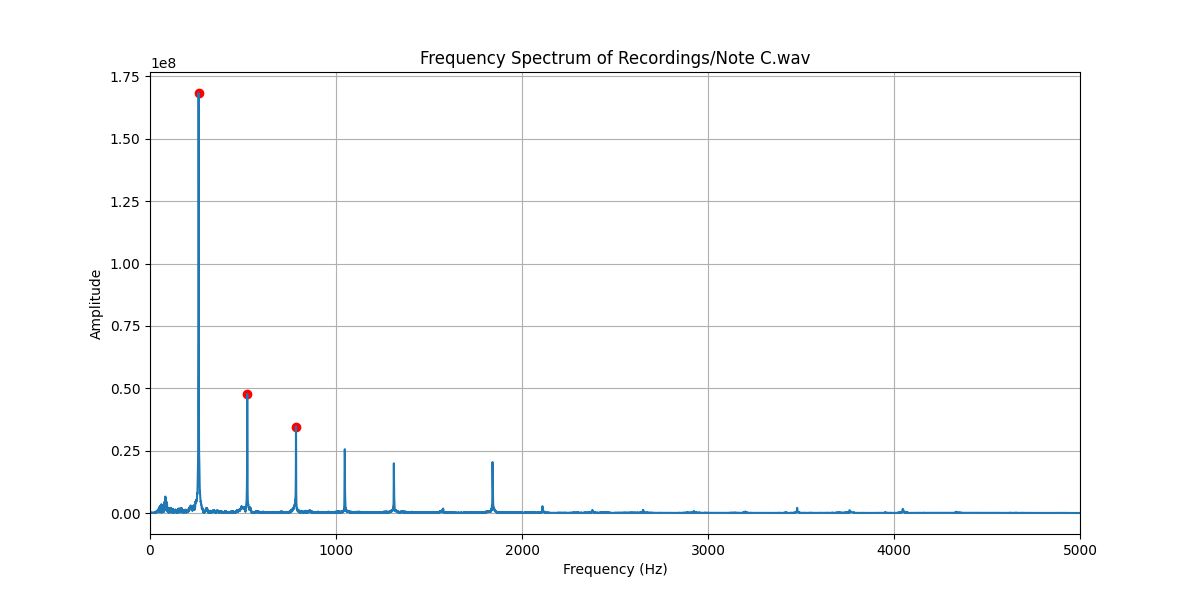
\includegraphics[width=\textwidth]{C Note.png}
        \caption{C}
        \label{fig:C4_Note}
    \end{subfigure}
    \begin{subfigure}{0.49\textwidth}
        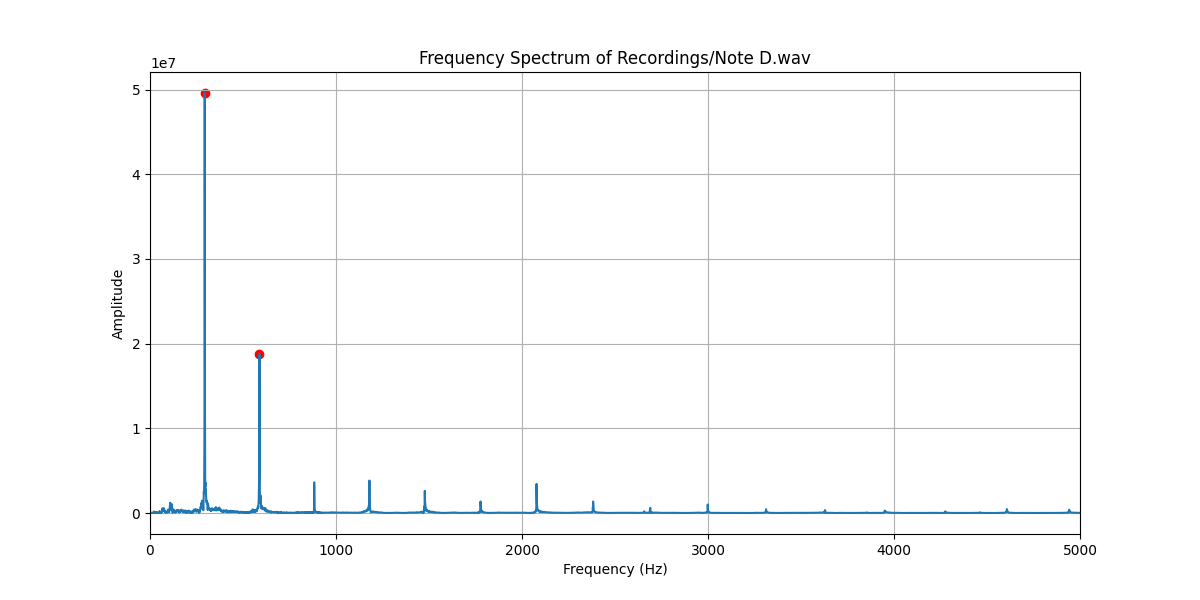
\includegraphics[width=\textwidth]{D Note.png}
        \caption{D}
        \label{fig:D4_Note}
    \end{subfigure}
    \begin{subfigure}{0.49\textwidth}
        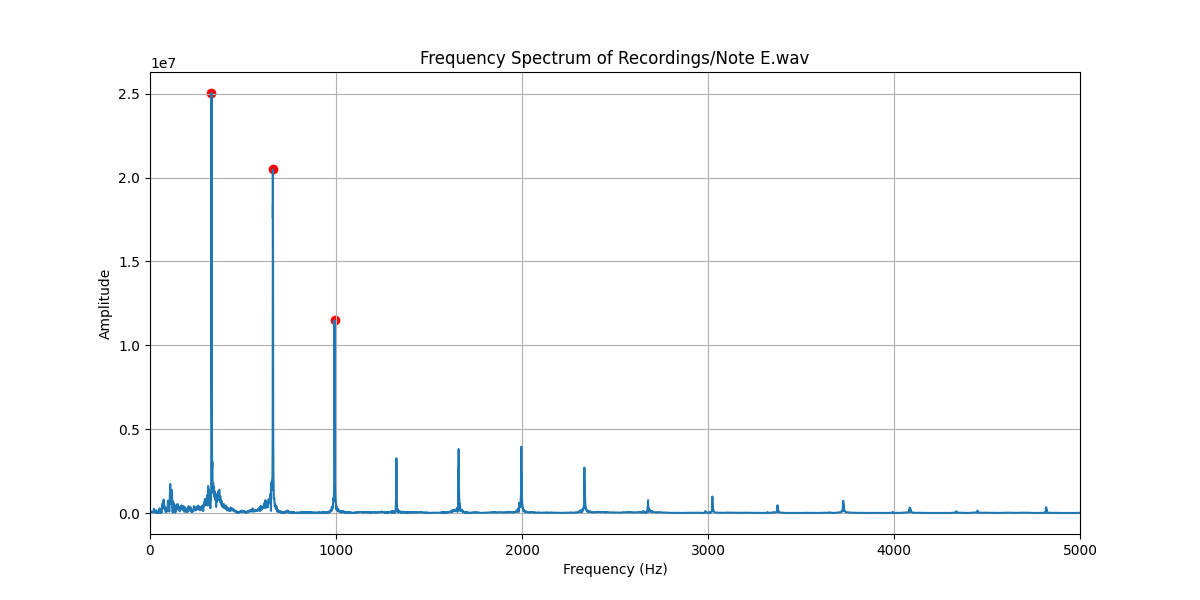
\includegraphics[width=\textwidth]{E Note.png}
        \caption{E}
        \label{fig:E4_Note}
    \end{subfigure}
        \label{fig:B4_Note}
        \begin{subfigure}{0.49\textwidth}
        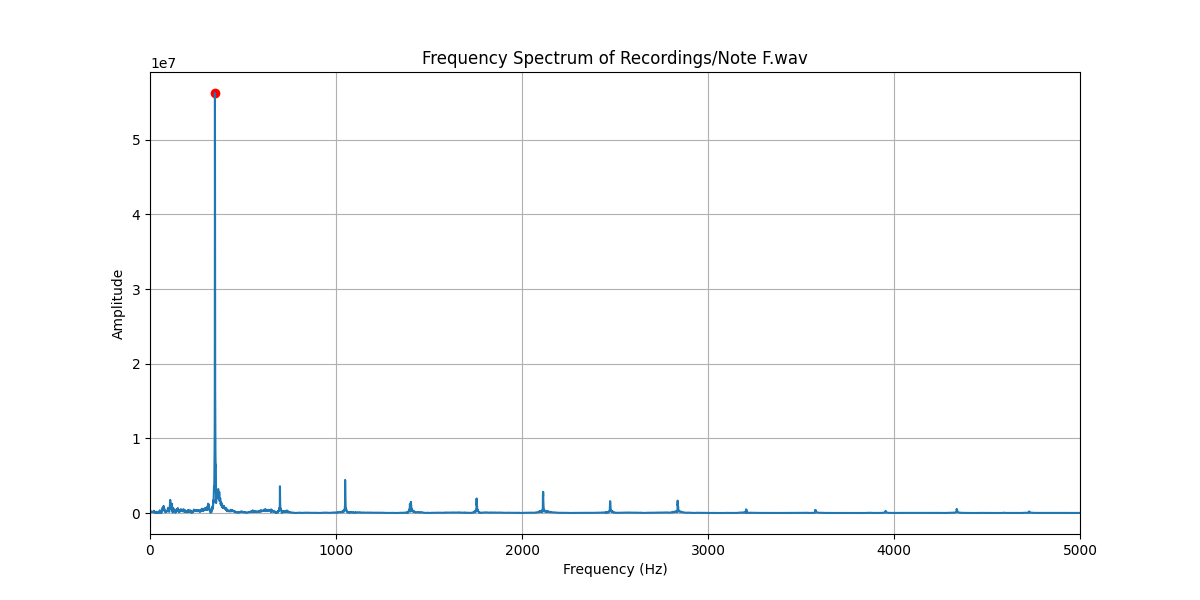
\includegraphics[width=\textwidth]{F Note.png}
        \caption{F}
        \label{fig:F4_Note}
    \end{subfigure}
     \centering
    \begin{subfigure}{0.49\textwidth}
        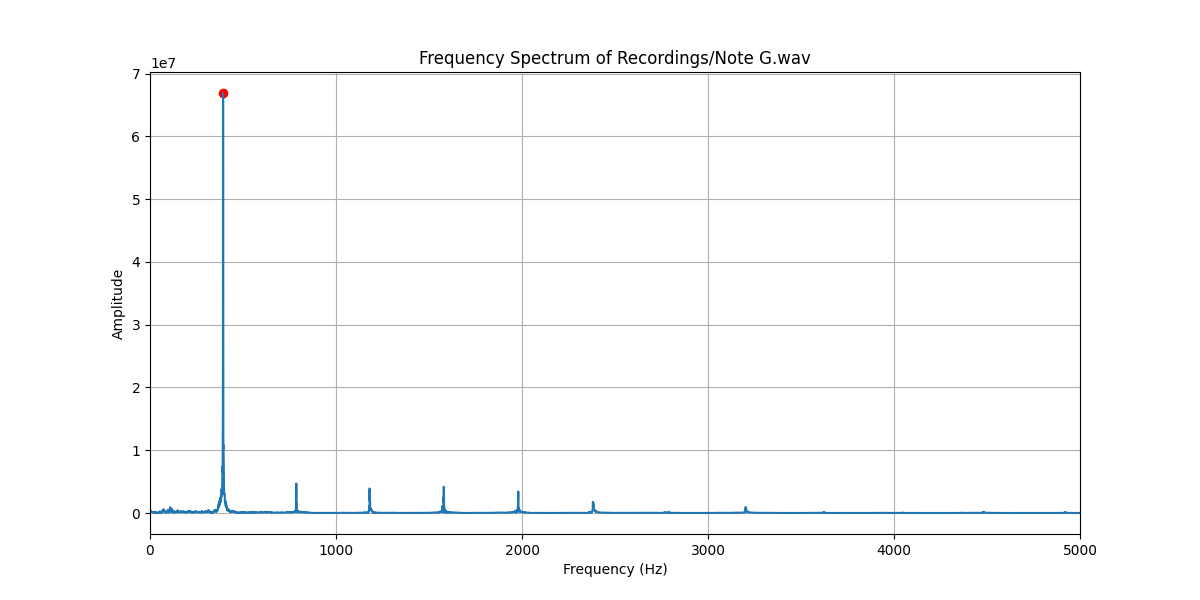
\includegraphics[width=\textwidth]{G Note.png}
        \caption{G}
        \label{fig:G4_Note}
    \end{subfigure}
    \begin{subfigure}{0.49\textwidth}
        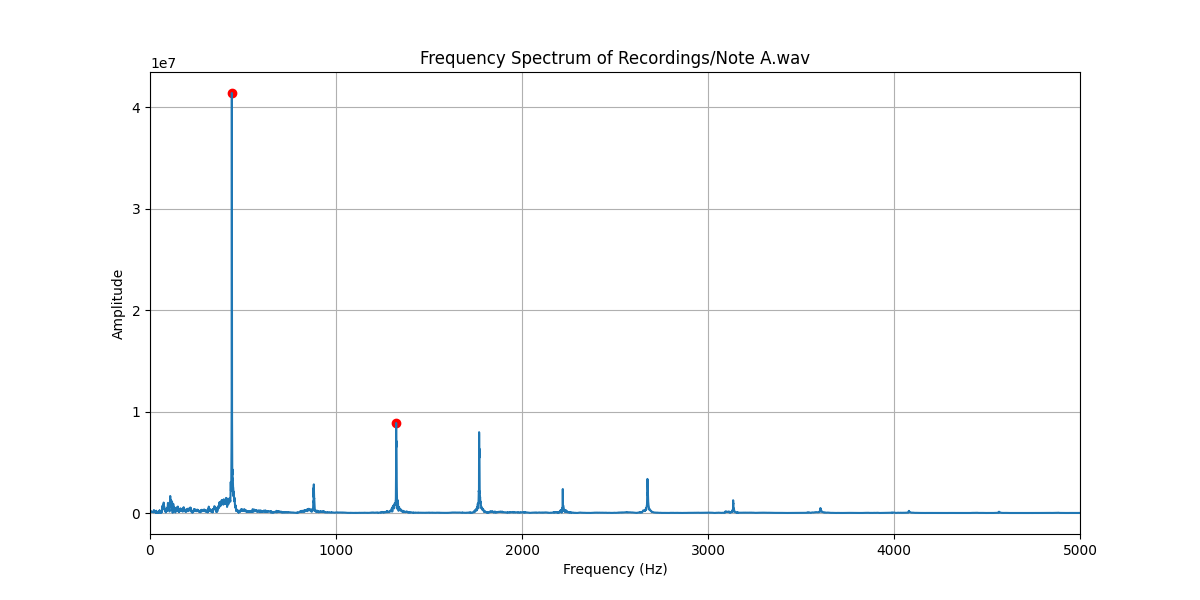
\includegraphics[width=\textwidth]{A Note.png}
        \caption{A}
        \label{fig:A4_Note}
    \end{subfigure}
    \begin{subfigure}{0.49\textwidth}
        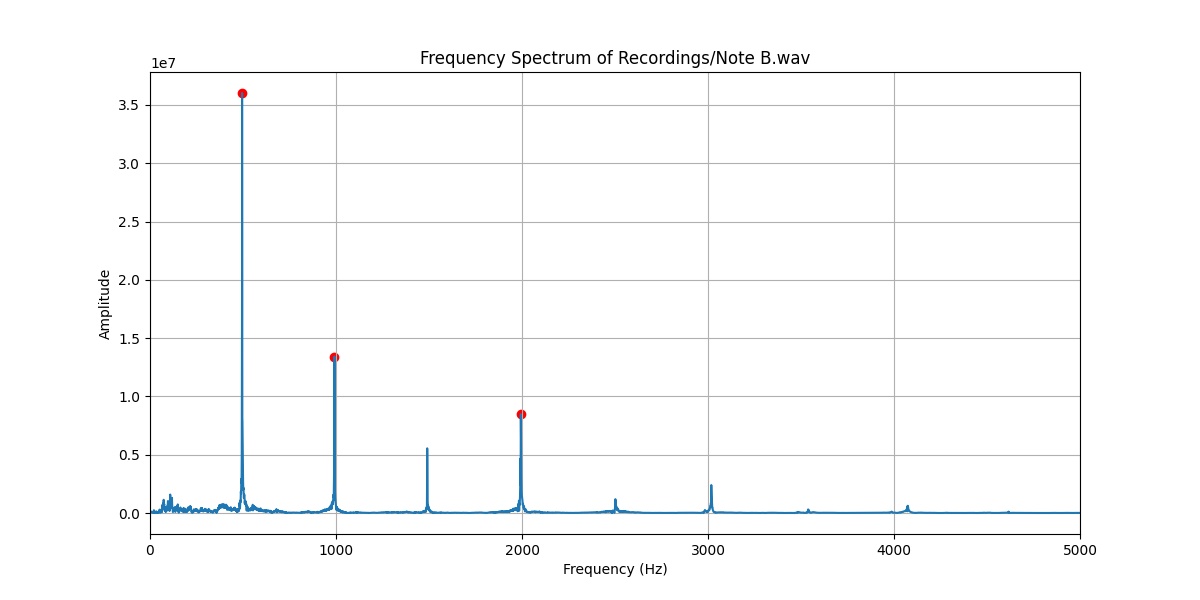
\includegraphics[width=\textwidth]{B Note.png}
        \caption{B}
        \label{fig:B4_Note}
    \end{subfigure}
    \caption{Musical Notes from C to B in the 4th Octave.}
    \label{fig:musical_notes}
    \end{figure}

It is evident that each note has only a few "strong" coefficients, while the majority are relatively "weak." By focusing on the coefficient with the most dominant amplitude, we observe that it corresponds to the frequency of the note: \\ C4: 261.6, D4: 293.7, E4: 329.6, F4: 349.2, G4: 392.0, A4: 440.0, B4: 493.9 Hz$^{[9]}$.\\\\
The fundamental frequencies identified during the analysis were:
C4: 261.36, D4: 294.20, E4: 330.48, F4: 349.03, G4: 393.02, A4: 439.99, B4: 495.12 Hz.

\item { \section* {Example of Use - Jingle Bells (Christmas song)}}

Therefore, we can Identify notes using the FFT in any audio recording. Take the Jingle Bells song (a Christmas song), that we have recorded manually, as an example: 

    \begin{figure}[H] 
    \centering
    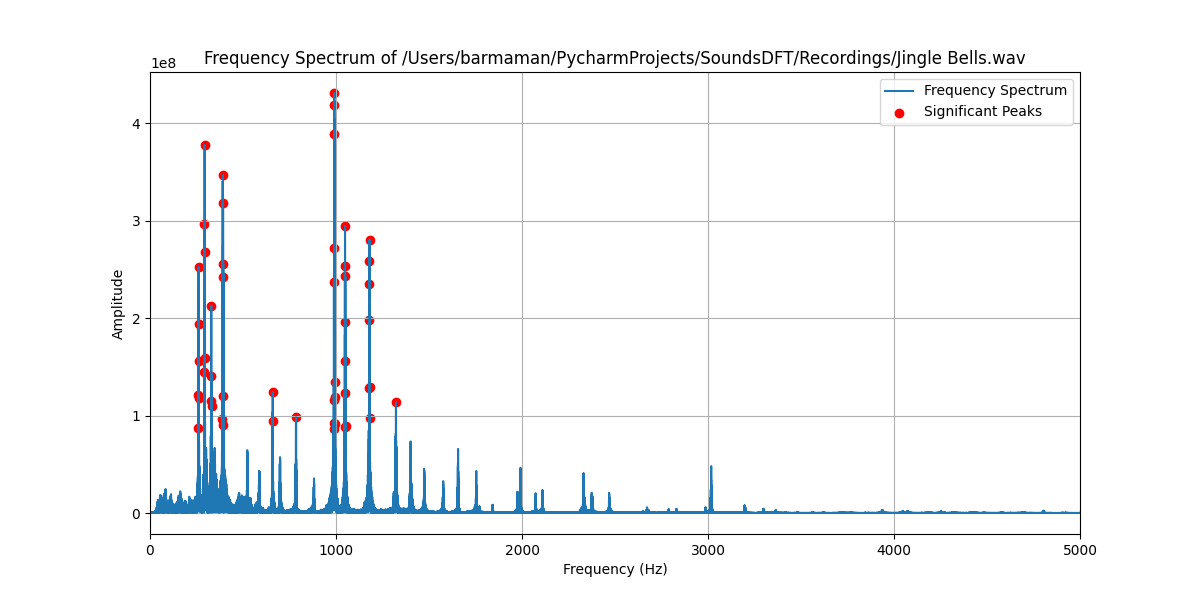
\includegraphics[width=0.8\textwidth]{Jingle Bells.png}
    \caption{graph of the recording of the Jingle Bells song coefficients}
    \label{fig:hat_function}
    \end{figure}

\item{ \section* {Tuning a Note}}
Using the ability to extract the dominant frequency of a recording, in this example we will demonstrate tuning the note C4:

We recorded a slightly untuned note which corresponds to 293.49 Hz, while the actual C4 Note corresponds to 261.63 Hz. After using the FFT akgorithm and extracting the dominant frequency we informed the user about the deviation from the Desired Reference Note, in our case C4: 

 \begin{figure}[H] 
    \centering
    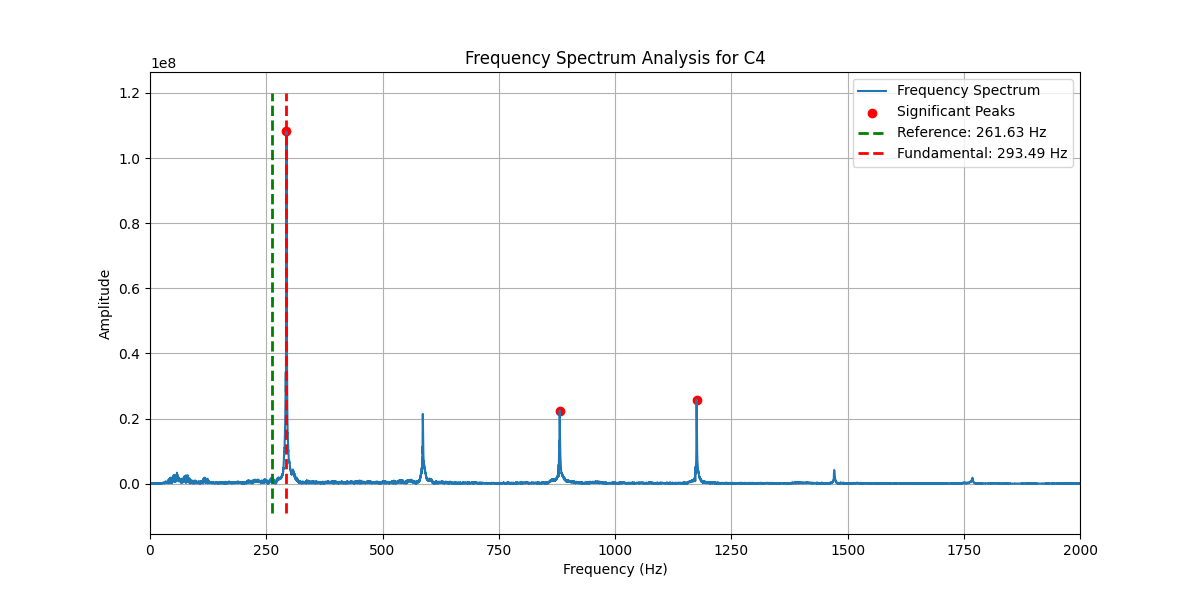
\includegraphics[width=0.8\textwidth]{TuneC4.png}
    \caption{Tuning a Note to C4}
    \label{fig:hat_function}
    \end{figure}

The output of the algorithm is the difference between the dominant frequency of the recording and the dominant frequency of the desired note. In the above example, it should be tuned down by 31.86

    

\end{itemize}
\section*{Conclusion}
The aim of our research was to develop a method for recognizing frequencies in audio recordings and tuning musical notes. Leveraging the wave-like behavior inherent in audio signals, we began with Fourier series analysis to decompose signals into their frequency components. However, we soon realized that calculating Fourier coefficients requires intensive computations. To address this challenge, we explained how to utilize matrix multiplication and dot product manipulations to project the signal onto the frequency domain, along with Euler's formula, to significantly reduce computational complexity.

This optimized approach allowed us to identify dominant frequencies in audio recordings more efficiently. Through a manual recording of each note, we observed that the most dominant frequency in the FFT output consistently corresponds to the natural frequency of a musical note in the real world. Building on this finding, we developed an algorithm that acts as a piano tuner. By analyzing a recorded note, the algorithm determines its dominant frequency and calculates the deviation from the target frequency, enabling precise tuning.

\section*{References}
\begin{enumerate}
    \item Brunton, Steven L., and J. Nathan Kutz. \textit{Data-Driven Science and Engineering}. University of Washington Press, 28 Feb. 2019.

    \item Stein, Elias M., and Rami Shakarchi. \textit{Fourier Analysis: An Introduction}. Princeton University Press, 2007.

    \item Smith, Julius O. \textit{Spectral Audio Signal Processing}. Stanford University, 2011. 
    \url{https://ccrma.stanford.edu/}

    \item J. W. Cooley, P. A. W. Lewis, and P. D. Welch, \textit{The Fast Fourier Transform and Its Applications}, in IEEE Transactions on Education, vol. 12, no. 1, pp. 27-34, March 1969. 
    \url{https://ieeexplore.ieee.org/abstract/document/4320436}

    \item Nikou, Christos. \textit{Audio Signal Processing and Audio Fingerprinting: Implementing a Music Recognition System.} Diploma thesis, National Technical University of Athens, School of Electrical and Computer Engineering, supervised by Konstantinos Karantzalos, co-supervised by Theodoros Giannakopoulos, MSc in Data Science \& Machine Learning, 2023. 
    \url{https://dspace.lib.ntua.gr/xmlui/bitstream/handle/123456789/59099/Nikou_DSML_Thesis.pdf?sequence=1}

    \item A. C. Gilbert, P. Indyk, M. Iwen, and L. Schmidt, \textit{Recent Developments in the Sparse Fourier Transform: A compressed Fourier transform for big data}, in IEEE Signal Processing Magazine, vol. 31, no. 5, pp. 91-100, Sept. 2014. 
    \url{https://ieeexplore.ieee.org/abstract/document/6879613}

    \item G. D. Clifford, \textit{Singular Value Decomposition \& Independent Component Analysis for Blind Source Separation}, unpublished manuscript, April 2000. 
    \url{https://www.mit.edu/~gari/teaching/6.222j/ICASVDnotes.pdf}

    \item Benko, Uroš, and Đani Juričić. "Frequency Analysis of Noisy Short-Time Stationary Signals Using Filter-Diagonalization." \textit{Signal Processing}, vol. 88, no. 7, 2008, pp. 1733--1746. \textit{ScienceDirect}, 
        \url{https://www.sciencedirect.com/science/article/pii/S0165168408000170}

    \item "Piano Key Frequencies." \textit{Wikipedia}, The Free Encyclopedia, 5 Dec. 2023, 
    \url{https://en.wikipedia.org/wiki/Piano_key_frequencies}.

\end{enumerate}

\section* {Code References}
\begin{minted}[frame=lines, fontsize=\small]{python}
def analyze_piano_note(file_path, note):
    sample_rate, data = wavfile.read(file_path)

    # Applying the FFT on the current note
    fft_vector_output = np.fft.fft(data)
    amplitudes_of_frequencies = np.abs(fft_vector_output)
    frequencies = np.fft.fftfreq(len(fft_vector_output), 1 / sample_rate)

    # Finding the most important frequencies
    threshold_relavive_amplitudes = np.max(amplitudes_of_frequencies) * 0.20
    peaks, qualities = find_peaks(amplitudes_of_frequencies[:len(frequencies) // 2], height=threshold_relavive_amplitudes, distance=20,
                                   prominence=0.05)

    if peaks.size > 0:
        fundamental_index_of_frequencies = peaks[np.argmax(amplitudes_of_frequencies[peaks])]
        fundamental_frequency = frequencies[fundamental_index_of_frequencies]
        print(f"The most Dominant frequency of {note}: {fundamental_frequency:.2f} Hz")

\end{minted}




\end{document}
